\section{Conclusions}
\label{sec:conclusions}

\begin{figure*}
  \centering
  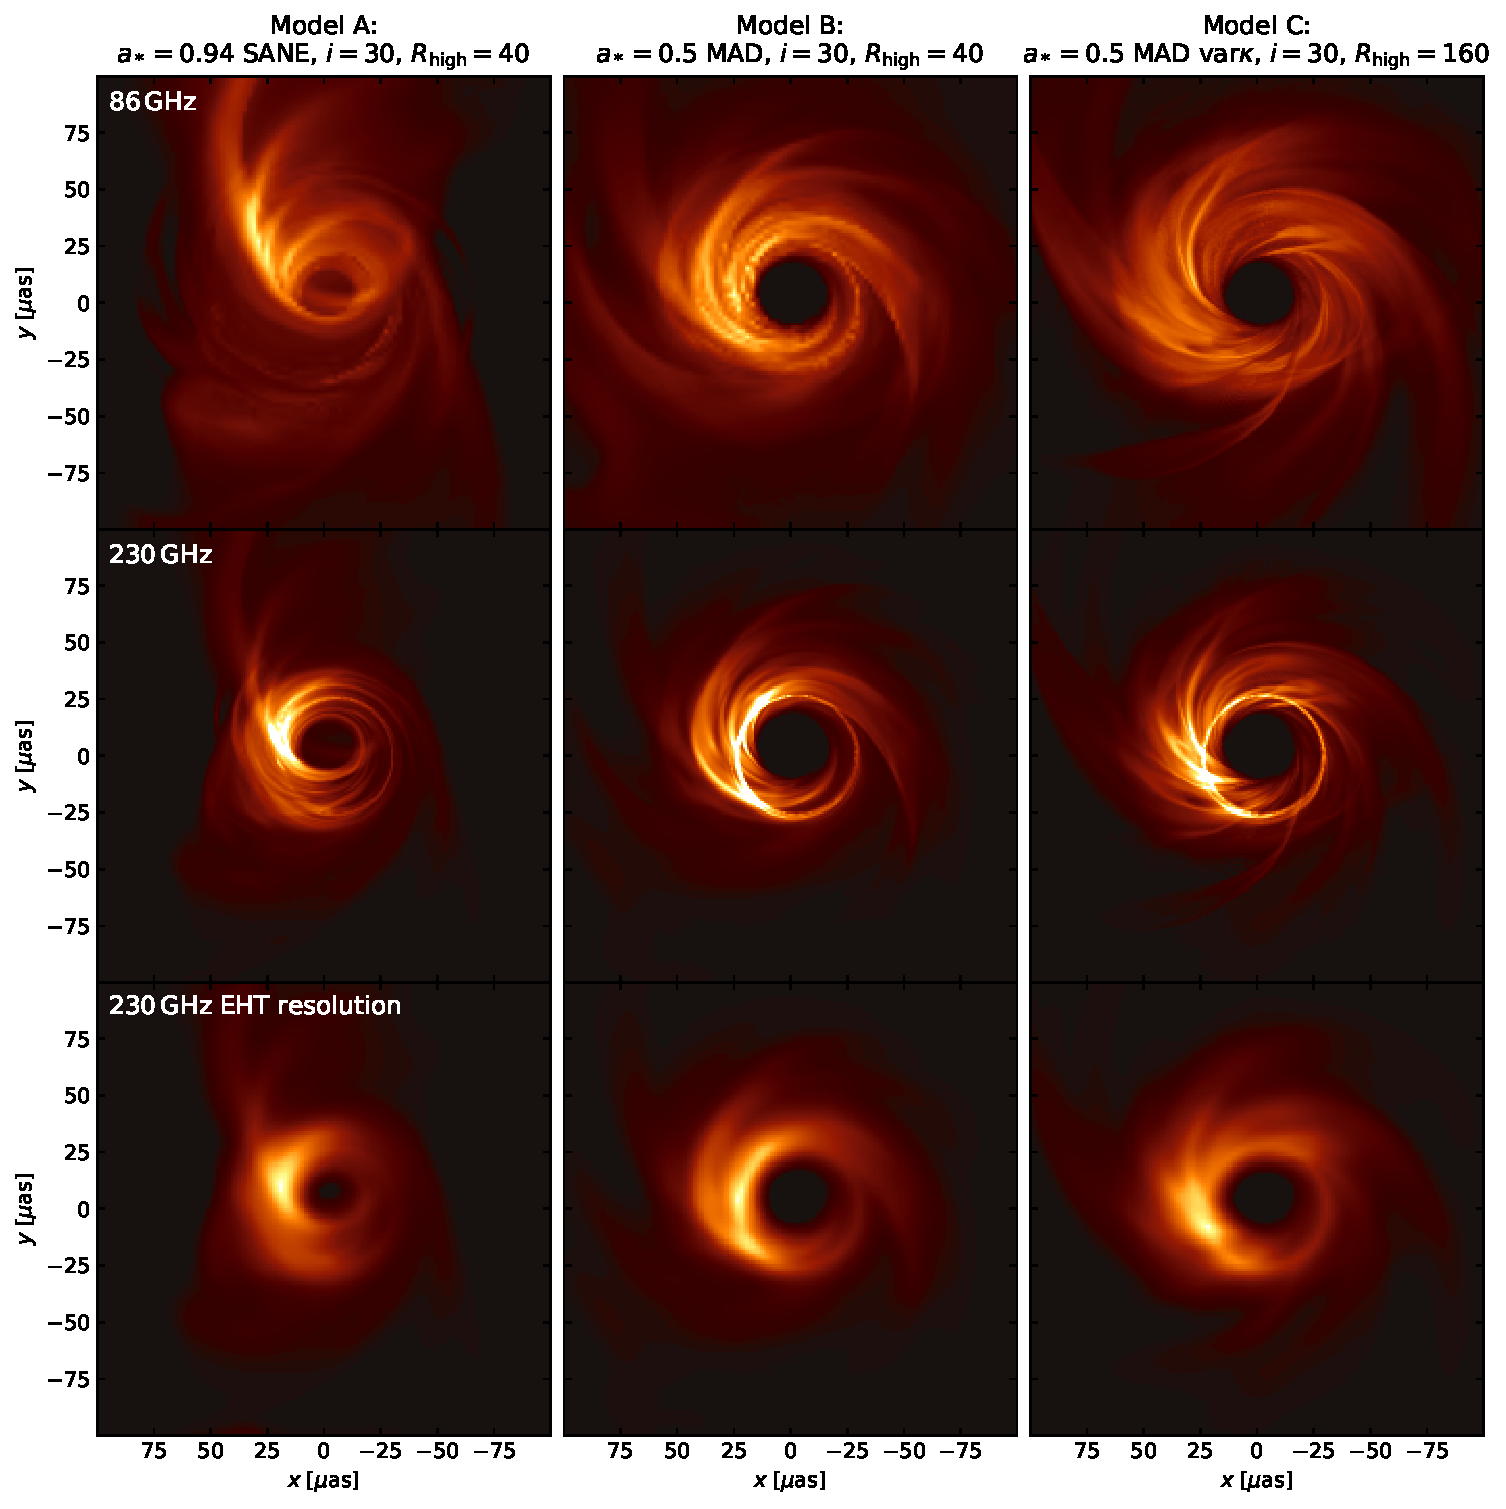
\includegraphics[width=\textwidth]{figures/bestbet_imgs.pdf}
  % cfg 15-dec: edited down
  \caption{Best bet model that pass 10/11 constraints.
    The leftmost panel shows its 86\GHz ray traced image.
    The subsequent panels are the 230\GHz ray traced image,
    the 230\GHz image convolved with a 20\uas FWHM Gaussian for approximating the image at EHT resolution, and
    the actual reconstructed image from the EHT 2017 observation.
    Note that the position angle is not well constrained.
    So the rotation of the image here for matching the observed image is not statistically meaningful.}
  \label{fig:bestbet_imgs}
\end{figure*}

We have made a first comparison of the EHT 2017 \sgra data to a state-of-the-art library of ideal general relativistic magnetohydrodynamics (GRMHD) models.  The models assume that the mass and distance to \sgra are known and that the central object is a black hole described by the Kerr metric.  We use multiple simulation pipelines and find that for a given set of initial and boundary conditions, independent simulations are remarkably consistent (see Appendix~\ref{app:numerical}).

The model parameters are: whether the horizon magnetic field is strong or weak (MAD or SANE, respectively); the black hole spin $\abh$; and the inclination angle $i$ between the line of sight and the black hole spin vector.  The electron distribution function (eDF) also has one or more parameters.  In our ``standard'' model set, run with three independent codes, the eDF is determined using the so-called $\Rh$ prescription (see Section \ref{sec:models}).  We have also considered non-standard models with alternate eDF prescriptions and alternate initial conditions.

We have selected and applied 11 heterogeneous observational constraints.  Six derive directly from EHT VLBI data, two derive from 86\GHz VLBI observations with the GMVA, one from variability of the 230\GHz lightcurve, and one each from the 2.2\um flux density and the x-ray luminosity.

Five structural constraints derive from EHT VLBI data.
While these constraints are not independent, which makes their interpretation as likelihood difficult, the multiple constraints make our analyses more robust.
When combined these constraints reject about 75\% of our standard models.  The EHT cut favors $\abh \ge 0$ and avoids edge-on ($i = 90\degree$) models and models with equal ion and electron temperatures ($\Rh = 1$).
We are {\em not} able to constrain the source position angle due to sparse baseline coverage.
The 2017 EHT observations are, nevertheless, quite constraining; new EHT observations with more baselines will be even more constraining.

Four constraints derive from non-EHT data that is contemporaneous or near-contemporaneous.  Combined, the non-EHT constraints reject 88\% of standard models.  The non-EHT cut favors strongly magnetized (MAD) models, eliminates all models with equal ion and electron temperatures, and eliminates most models at $i > 50\degree$.  These results highlight the value of continued multiwavelength monitoring of \sgra.

\sgra is variable.  We have used two tests to compare the variability of models and data. One characterizes variability in the 230\GHz lightcurve (including simultaneous ALMA data) and the other structural characterizes variability expressed through fluctuations in the visibility amplitudes.  The lightcurve variability is the tightest of all 11 constraints: it rejects 77\% of our standard models.  We find that strongly magnetized (MAD) models are more variable than weakly magnetized (SANE) models and, grouped together, both SANE and MAD models are more variable than the data.  The structural variability measures the slope and amplitude of the visibility amplitude power spectrum.  Remarkably, we find that the power spectrum slope is consistent for all models, while the power spectrum amplitude is inconsistent for 34\% of standard models.

The failure of most standard models to match the lightcurve variability is interesting.  It may signal the presence of extended, slowly varying structure that is resolved out by EHT, or it may signal that future models need to incorporate collisionless effects (potentially modeled as viscosity and conductivity) or a more sophisticated treatment of electron thermodynamics including cooling.  If each of these effects reduces $\mi{3}$ by about $10\%$ then many of the MAD models would be consistent with the data.

None of the standard models survive the full gauntlet of 11 constraints.
If we set aside variability, however, there is a cluster of 3 models that pass the remaining 10 constraints in both the Illinois and Frankfurt standard models (a few more survive in one model set but not the other).  These ``best-bet'' models are are strongly magnetized (MAD) and have $\Rh = 160$, positive spin, and low inclination ($\abh, i = 0.5, 30; 0.94, 10; 0.94; 30$).  Images of the best-bet models are shown in Figure \ref{fig:bestbet_imgs}, along with the observed image.


Our cluster of best-bet models has accretion rate $\dot{M} = 5.2$--$9.5 \times 10^{-9}\msun\yr^{-1}$.
These accretion rates are consistent with earlier estimates and overlap with accretion rates in wind-fed models, $\sim 10^{-8} \msun\yr^{-1}$ \citep{2020ApJ...896L...6R}.
The $\abh = 0.5$ MAD with $i=30$ model is presented in Figure~\ref{fig:bestbet_imgs}, together with a smoothed image that matches the EHT resolution and one of the reconstruction from the 2017 EHT observation.

We produced synthetic SEDs, and therefore bolometric luminosities $L_\mathrm{bol}$, for all standard models.  Typically $L_\mathrm{bol}$ is dominated by a synchrotron bump in the submm and for the best-bet models is $6.8$--$9.8\times10^{35}\ergps$; the corresponding radiative efficiency $L_\mathrm{bol}/(\dot{M} c^2)$ is $1.3$--$3.0\times 10^{-3}$.  The maximum radiative efficiency over the entire standard model set is 0.08 (for a MAD, $\abh = 0.94$, $\Rh = 1$ model), which is necessary but not sufficient to justify our neglect of radiative cooling in the GRMHD evolution.

All our models produce bipolar outflows, and for each we measured the outflow power $P_\mathrm{out}$, defined in Section~\ref{sec:discussions}. Consistent with earlier work we find that outflow power is higher for strongly magnetized (MAD) models than for comparable weakly magnetized (SANE) models, and increases by more than an order of magnitude from $\abh = 0$ to $|\abh| = 0.94$.  For the best-bet models $P_\mathrm{out} = 1.3$--$4.8 \times 10^{38}\ergps$, corresponding to an outflow efficiency $P_\mathrm{out} /(\dot{M} c^2)$ of 0.25--1.6.  Such large  outflow efficiency is only possible if energy is extracted from a spinning black hole via the mechanism proposed by  \cite{1977MNRAS.179..433B}.  It is an open question how these powerful outflows might interact with incoming gas in a self-consistent accretion model that follows plasma over a larger range in radius than our standard models.  It is also an open question whether the outflow power could be detected in the dense but crowded galactic center environment.  Notice that this outflow luminosity is comparable to the spindown luminosity of the Crab pulsar.

Our standard models assume a particular parameterization for the electron distribution function (the $\Rh$ prescription), use a common initial setup (a magnetized torus), and assume the black hole spin vector and torus angular momentum are aligned or anti-aligned.  To partially control for the errors introduced by these assumptions we have explored a set of nonstandard models.  The nonstandard models include several eDF prescriptions, a wind-fed model that tracks accretion from stellar winds down to the scale of the horizon, and tilted disk models in which the black hole spin and torus angular momentum are misaligned.

Our nonthermal models do not differ significantly from their thermal counterparts.
% cfg 15 dec: I agree with this, but I think readers would find it confusing since we normalized all our models at 230.
%\ckc{... because we normalize $\mathcal{M}$ by setting the 230\GHz flux to 2.4\,Jy; if we were, for example, set the normalization by fixing the x-ray flux, then the nonthermal models will lead to significant different 230\GHz images.  One possible conclusion is that, this study shows determining the density unity from emission near the emission peak is a good strategic to study supermassive black holes.}
For the limited set of nonthermal eDF prescriptions we consider here the 230\GHz image structure differs very little.
The 230\GHz variability is not detectably different than corresponding thermal models.\footnote{The nonthermal models are imaged over $5\times 10^3\tg$, so constraints on $\mi{3}$ are weaker than for the standard models, which are imaged for 3 times as long.}
The 86\GHz size and flux density, which are the most restrictive non-EHT constraints, are not detectably affected by the addition of nonthermal electrons for most nonthermal models (except $\kappa = 5$ models).
Nonthermal electrons consistently increase the 2.2\um flux density over similar thermal models, however.
Accelerating even a small fraction of the electron population into a nonthermal tail risks overproducing 2.2\um emission.
The 2.2\um (and submm through mid-IR) flux density therefore provides the strongest eDF constraints.
Future EHT analyses would benefit from incorporating submm constraints \citep[e.g.][]{2019ApJ...881L...2B} and, because model submm SEDs are highly variable, the submm and 2.2\um data should be near-simultaneous as possible.

The stellar wind-fed models of \cite{2020ApJ...896L...6R} feature the best-motivated treatment of boundary and initial conditions for \sgra models.  They differ from our torus-initialized standard models in that they follow plasma from its ejection from stars on known orbits down to the event horizon.  We have imaged these models using an $\Rh$ prescription for the electron temperature, with $\Rh$ adjusted in the otherwise parameter-free models to produce the correct time-averaged 230 GHz flux density.  The two models considered here, both with $\abh = 0$, fail the 86\GHz flux, \mring width, and $\mi{3}$ constraints.  This does {\em not} imply that wind fed models are ruled out; they clearly merit further investigation with longer integrations over a broader range of eDFs and $\abh$.

In general, black hole accretion flows can be tilted in the sense that the orbital angular momentum of the disk and the spin angular momentum of the hole are misaligned.  Tilted disks have not been included in EHT analyses because \emph{i}) it is conceivable that accretion flows align either by consistently oriented long term accretion or by some analog of the Bardeen-Petterson effect \citep{1975ApJ...195L..65B} and \emph{ii}) the tilted disk parameter space is larger than the aligned disk parameter space by two dimensions: the tilt angle and the longitude of the observer.  We considered models with tilt $30\degree$ and $60\degree$, observed at a single longitude.  The integrations were too short ($3000\tg$) to provide strong constraints on tilt, but we find that the \mring width test is particularly sensitive to tilt and rejects a progressively larger fraction of the models as tilt increases at the single observing longitude studied here.  Tilted models clearly merit further investigation.

Our standard models and variable $\kappa$ nonthermal models have been run with independent GRMHD codes and imaged with independent radiative transfer codes.  The outcomes are largely consistent (see Appendix~\ref{app:numerical} for details).  The code comparisons were valuable and helped us identify, for example, the importance of a large field of view in 86\GHz imaging.  The consistency between codes is remarkable given the complexity of the modeling process and the scope for error.  Tracking down the remaining discrepancies (for example, in the 2.2\um flux density) and developing a quantitative error budget is an essential but difficult task for the future.

This first comparison of the EHT 2017 \sgra data to state-of-the-art GRMHD models shows remarkable successes and highlights interesting problems, including the origin of variability.  The observational constraints considered here put pressure on the theoretical models, and the models are not trivially adjustable to pass all tests.  This work signals the arrival of a new era of precision black hole astrophysics in which close interaction of theory and experiment has the potential to unveil the inner workings of the galactic center.
